%!TEX root = ../Angebot.tex

\chapter{Projektablauf}

\section{Meilensteine}

Alle wichtigen Ereignisse, wie zum Beispiel Abgabefristen die vom Kunden oder der Projektleitung gesetzt werden, aber auch intern im Team gesetzte Fristen, werden 
in Meilensteinen zusammengefasst und in einer Tabelle wiedergegeben. Dabei ist bei jedem einzelnen Meilenstein jeweils die Vervollst\"andigung gemeint.
Jedes Dokument wird vor jeder offiziellen Abgabe dem Betreuer zur Kontrolle vorgelegt.

\begin{longtable}{|l|c|c|c|c|}
	\hline
	\textbf{Nummer} & \textbf{Meilenstein} & \textbf{Dokumente} & \textbf{Abgabetermin}\\ 
	\hline
	1  	&  Projektstart      &         -     &    13.04.15     \\ 
	\hline
	2	&  Angebot an Betreuer & Angebot & 20.04.15 \\
	 \hline
	3	& Serverapplikation initialisiert & - & 24.04.15 \\
	\hline
	4	& Angebot \"uber Redmine & Angebot & 24.04.15 \\
	\hline
	5	& Vervollst\"andigen der Spielidee &  - & 24.04.15 \\
	\hline
	6 	& Pflichtenheft an Betreuer &  Pflichtenheft & 06.05.15 \\ 
	\hline
	7 	& GUI des Front-Ends  & - & 07.05.15 \\
	\hline
	8 	& Userverwaltung & - & 07.05.15 \\
	\hline
	9 	& Pflichtenheft \"uber Redmine &  Pflichtenheft & 13.05.15 \\
	\hline
	10 	& Zwischenpr\"asentation  &  - & 15.05.15 \\
	\hline
	11 	& Fachentwurf an Betreuer &  Fachentwurf & 27.05.15 \\
	\hline
	12 	& Fachentwurf \"uber Redmine &  Fachentwurf & 03.06.15 \\	
	\hline
	13 	& Verwaltung f\"ur Benutzerrechte & - & 24.06.15 \\
	\hline
	14 	& Technischer Entwurf an Betreuer &  Technischer Entwurf & 24.06.15 \\
	\hline
	15 	& Softwaretests & - & 30.06.15 \\
	\hline
	16 	& Technischer Entwurf \"uber Redmine &  Technischer Entwurf & 01.07.15 \\
	\hline
	17 	& Fertigstellung Minigame & - & 24.06.15 \\
	\hline
	18 	& Testdokumentation an Betreuer &  Testdokumentation & 08.07.15 \\
	\hline
	19 	& Testdokumentation \"uber Redmine &  Testdokumentation & 15.07.15 \\
	\hline
	20 	& Pr\"asentationsvorbereitung & - & 20.07.15 \\
	\hline
	21 	& Fertige Version &  Quellcode, ... & 23.07.15 \\
	\hline
\end{longtable}

\section{Geplanter Ablauf}

Ein Teil des Teams startet das Projekt mit dem Ausformulieren des Produktangebots. W\"ahrenddessen beginnt das Gestaltungsteam ihren kreativen Prozess.
Ideenentwicklung und -austausch sowie N\"utzlichkeitsabw\"agung f\"uhren schnell zur fertigen Spielidee. Dieser Ablauf wird gleichzeitig genutzt, um zu pr\"ufen welche 
Werkzeuge (Frameworks, Entwicklungsumgebungen, etc.) genutzt werden, und sich mit diesen vertraut zu machen. Dabei werden auch schon erste Grafiken wie etwa 
f\"ur den Start-Screen und das Hauptmen\"u enstehen.

Das Back-End-Team nutzt die Zeit um die Serverapplikation zu erstellen. Desweiteren werden Ideen f\"ur ein Administrationstool sowie zur User- und Datenverwaltung 
gesammelt und umsetzbar strukturiert. Zwischenzeitig wird ein Papierprototyp entstehen, der die Grundz\"uge der zu erstellenden Applikation enth\"alt und das Team auf
einen gemeinsamen Stand bringt.

Sobald der Kunde, sowie der Betreuer das Angebot angenommen haben, beginnt der praktische Teil.

Das n\"achste Ziel wird sein, einen lauff\"ahigen Prototypen zu entwickeln.
Daf\"ur erstellen ausgew\"ahlte Mitglieder des Entwicklerteams das sogenannte Pflichtenheft, um festzuhalten, was von dem Projektteam alles geliefert werden muss.
Bis zur Fertigstellung des Prototypen und dessen Pr\"asentation wird weiterhin ein Fachentwurf erstellt und eingereicht.

Das Front-End-Team wird nun sowohl das Hauptmen\"u als auch das \glqq Alchemistenlabor\grqq~(den eigentlichen \glqq SQL-Vokabeltrainer\grqq) bearbeiten, damit der repr\"asentative 
Teil des Projekts m\"oglichst zur Zwischenpr\"asentation ausf\"uhrbar ist.
Parallel wird sich das Back-End-Team um die Nutzer- und Rechteverwaltung k\"ummern. 

Nach der Zwischenpr\"asentation werden der Projektdokumentation noch der Technische Entwurf und die Testprotokolle hinzugef\"ugt.
Um die dazugeh\"origen Software-Tests k\"ummert sich das Team in der letzten Etappe.

Zum Abschluss des Projektes wird eine kleinere Gruppe aus ausgew\"ahlten Mitgliedern noch f\"ur eine gute Pr\"asentation beim Tag der jungen Software-Entwickler 
(TDSE)  sorgen. 

Zur besseren \"Ubersicht dieser einzelnen Abl\"aufe ist ein Gantt-Diagramm erstellt worden.

\begin{figure}[ht]
\centering
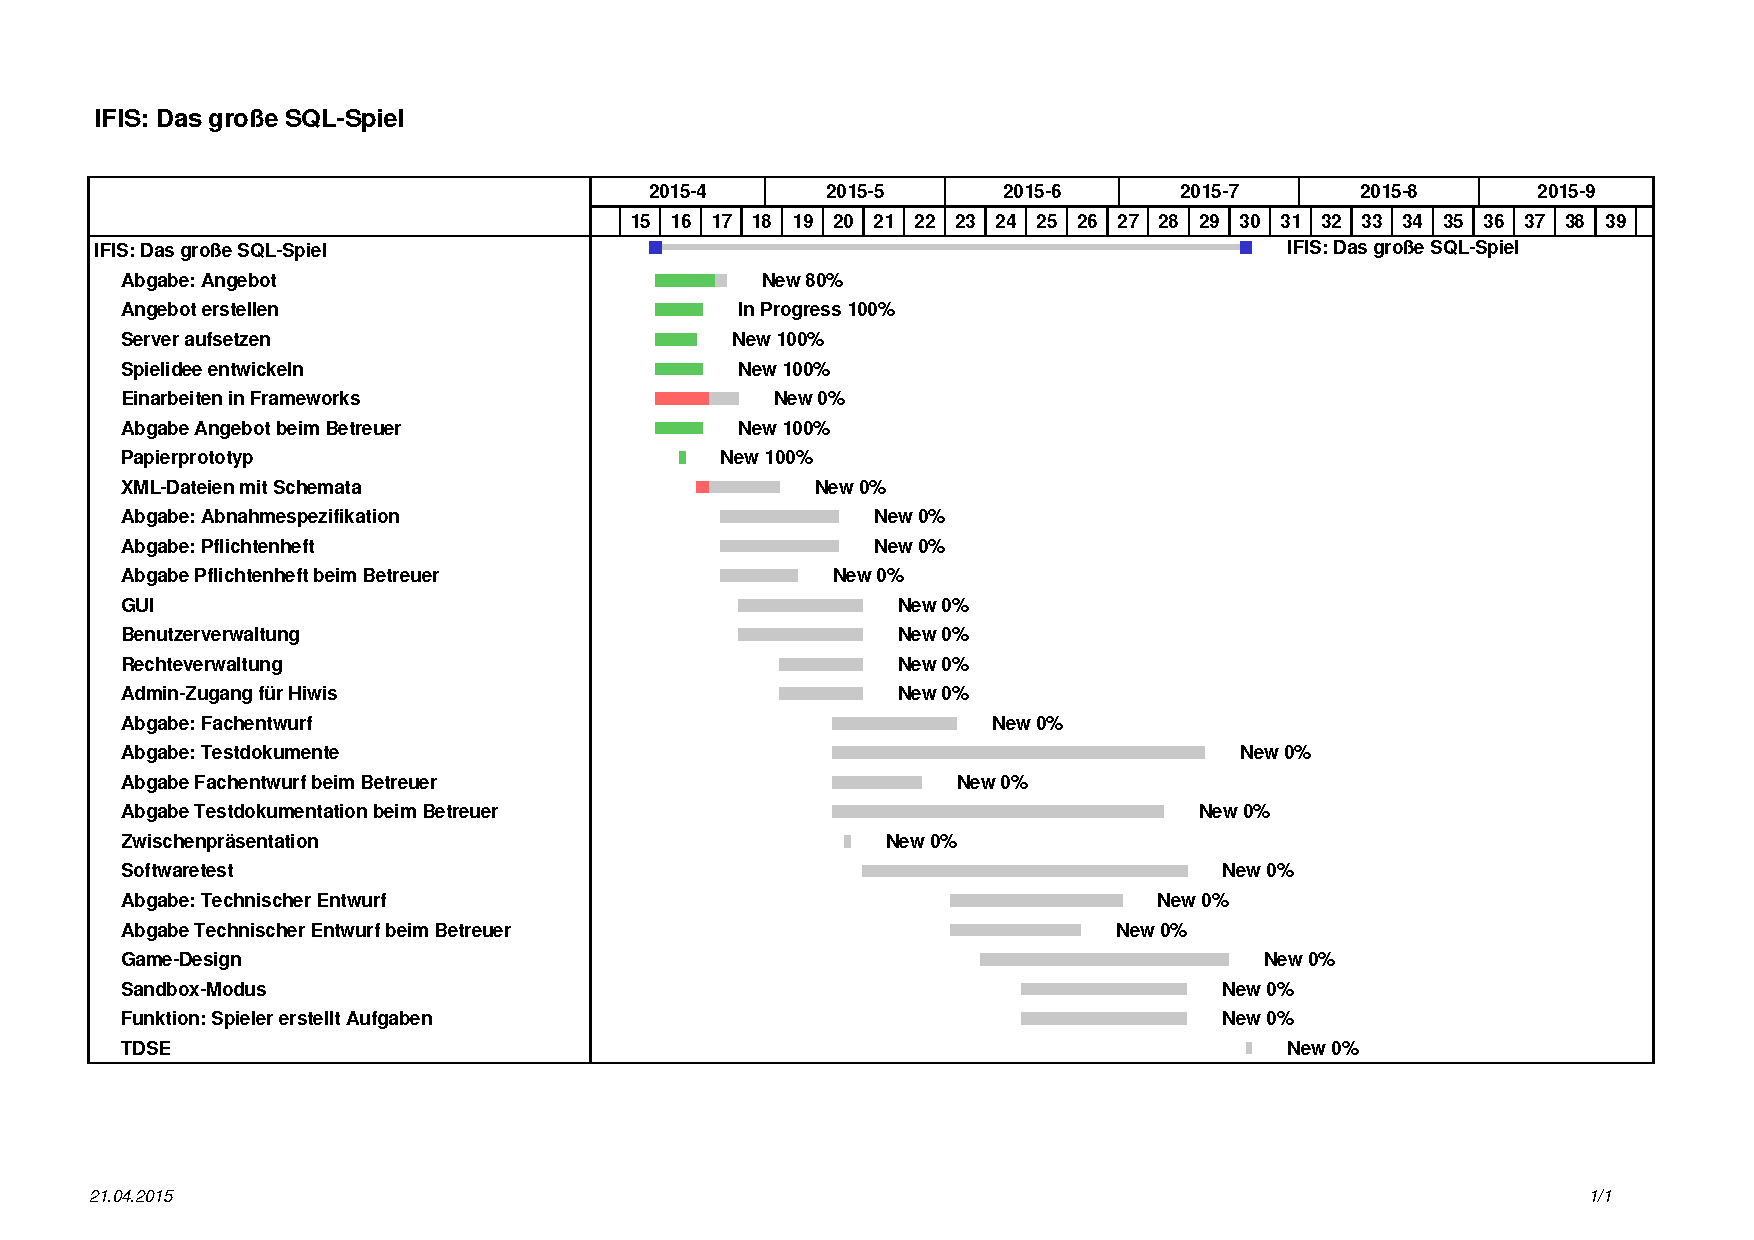
\includegraphics[height=\textwidth, angle=90]{figures/gantt.pdf}
\caption{Gantt-Diagramm}
\label{gantt}
\end{figure}